\documentclass[svgnames,11pt]{beamer}
\input{/home/tof/Documents/Cozy/latex-include/preambule_commun.tex}
\input{/home/tof/Documents/Cozy/latex-include/preambule_beamer.tex}
%\usepackage{pgfpages} \setbeameroption{show notes on second screen=left}
\author[]{Christophe Viroulaud}
\title{Ordonnancement - implémentation}
\date{\framebox{\textbf{Archi 05}}}
%\logo{}
\institute{Terminale - NSI}

\begin{document}
\begin{frame}
    \titlepage
        \note{\fcolorbox{black}{red}{{\LARGE ordonnancement.zip sur site}}}
\end{frame}
\begin{frame}
    \frametitle{}

    Le processeur peut adopter plusieurs stratégies pour exécuter l'enchaînement des processus. Selon l'algorithme utilisé la structure adoptée pour stocker la liste des tâches a une importance fondamentale.
    \note{First Come First Served, Shortest Job First\dots}
\end{frame}
\begin{frame}
    \frametitle{}

    \begin{framed}\centering
        Quelles structures de données adopter pour implémenter les algorithmes d'ordonnancement?
    \end{framed}
    \note{Il est possible de construire plusieurs structures tirant avantage du principe de la liste chaînée}
\end{frame}
\section{Des structures héritées de la liste chaînée}
\subsection{Pile}
\begin{frame}
    \frametitle{Pile}
    \begin{aretenir}[]
        Les piles (\emph{stack}) sont fondées sur le principe du \emph{dernier arrivé premier sorti} : \textbf{L}ast \textbf{I}n \textbf{F}irst \textbf{O}ut.
    \end{aretenir}


\end{frame}
\begin{frame}
    \frametitle{}

    \begin{center}
        \begin{tikzpicture}[scale=0.5]
            \draw (0,0) grid (1,3);
            \draw (-2,4) grid (-1,5);

            \draw[->,>=latex] (-1,4.5) to[out=0,in=90] (0.5,3);

            \draw (5,0) grid (6,3);
            \draw (7,4) grid (8,5);

            \draw[->,>=latex] (5.5,3) to[out=90,in=180] (7,4.5);
        \end{tikzpicture}
        \captionof{figure}{Empiler - dépiler}
    \end{center}
    \note{pile d'assiettes}
\end{frame}
\begin{frame}
    \frametitle{}

    \begin{center}
    

        \begin{tikzpicture}[scale=0.6]
            \foreach \v/\y in {2/8,5/6,3/4,9/2}{
            \node[draw,minimum height=0.5cm] at (0,\y) {\v};
            \draw[->,>=latex] (0,\y-.5) -- (0,\y-1.5);
            }  
            \node at (0,0) {fin};  
            \node (s) at (4,8) {sommet};
            \draw[->,>=latex] (s) -- (0.5,8);
        \end{tikzpicture}
        \captionof{figure}{Implémentation}
    \end{center}
\end{frame}
\begin{frame}
    \frametitle{Interface d'une pile}
    Une pile stocke des éléments de type \textbf{\texttt{T}} quelconque.
    \begin{itemize}
        \item \texttt{\textbf{creer\_pile() $\rightarrow$ Pile()}}: crée une pile vide
        \item \texttt{\textbf{est\_vide(p: Pile) $\rightarrow$ bool}}: renvoie \textbf{\texttt{True}} si la pile est vide, \textbf{\texttt{False}} sinon.
        \item \texttt{\textbf{empiler(p: Pile, e: T) $\rightarrow$ None}}: ajoute un élément \emph{e} au sommet de la pile.
        \item \texttt{\textbf{depiler(p: Pile) $\rightarrow$ T}}: retire et renvoie l'élément du sommet de la pile.
    \end{itemize}

\end{frame}
\begin{frame}
    \frametitle{Implémentation}
    \begin{itemize}
        \item \texttt{\textbf{creer\_pile() $\rightarrow$ Pile()}}
        \item \texttt{\textbf{est\_vide(p: Pile) $\rightarrow$ bool}}
        \item \texttt{\textbf{empiler(p: Pile, e: T) $\rightarrow$ None}}
        \item \texttt{\textbf{depiler(p: Pile) $\rightarrow$ T}}
    \end{itemize}

    \begin{activite}
        La programmation orientée objet est un paradigme adapté pour implémenter une pile.
        \begin{enumerate}
            \item Créer une classe \textbf{\texttt{Element}}. Son constructeur initialisera deux attributs:
                  \begin{itemize}
                      \item \textbf{\texttt{donnees: int}}
                      \item \textbf{\texttt{successeur: Element}}
                  \end{itemize}
            \item \underline{Adapter l'interface} présentée pour créer une classe \textbf{\texttt{Pile}}.
            \item \textbf{Pour les plus avancés:} Implémenter la méthode \textbf{\texttt{\_\_str\_\_}} qui affiche le contenu de la pile.
            \item Quelle fonctionnalité du navigateur web utilise une pile?
        \end{enumerate}
    \end{activite}

\end{frame}
\begin{frame}[fragile]
    \frametitle{Correction}

    \begin{lstlisting}[language=Python , basicstyle=\ttfamily\small, xleftmargin=2em, xrightmargin=2em]
class Element:
    def __init__(self, d: int, s: object):
        self.donnees = d
        self.successeur = s
\end{lstlisting}
\end{frame}
\begin{frame}[fragile]

    \begin{lstlisting}[language=Python , basicstyle=\ttfamily\small, xleftmargin=2em, xrightmargin=2em]
class Pile:
    def __init__(self):
        self.sommet = None

    def est_vide(self) -> bool:
        return self.sommet is None
\end{lstlisting}
\end{frame}
\begin{frame}[fragile]

    \begin{lstlisting}[language=Python , basicstyle=\ttfamily\small, xleftmargin=2em, xrightmargin=2em]
def empiler(self, e: int) -> None:
    self.sommet = Element(e, self.sommet)
\end{lstlisting}
\end{frame}
\begin{frame}[fragile]

    \begin{lstlisting}[language=Python , basicstyle=\ttfamily\small, xleftmargin=1em, xrightmargin=1em]
def depiler(self) -> int:
    # gestion d'erreur
    if not self.est_vide():
        # récupère la valeur du haut de la pile
        res = self.sommet.donnees
        # retire le sommet
        self.sommet = self.sommet.successeur
        return res
\end{lstlisting}
\end{frame}
\begin{frame}[fragile]

    \begin{lstlisting}[language=Python , basicstyle=\ttfamily\small, xleftmargin=2em, xrightmargin=2em]
def __str__(self):
    affiche = ""
    last = self.sommet
    while last is not None:
        affiche += str(last.donnees) + "\n"
        last = last.successeur
    return affiche
\end{lstlisting}
\end{frame}
\begin{frame}
    \frametitle{}

    \begin{center}
        La fonction \textbf{retour} du navigateur web est un exemple de pile.\\
        La fonction \textbf{annuler} du traitement de texte également.
    \end{center}

\end{frame}
\subsection{File}
\begin{frame}
    \frametitle{File}

    \begin{aretenir}[]
        Les files (\emph{queue}) sont fondées sur le principe du \emph{premier arrivé premier sorti}: \textbf{F}irst \textbf{I}n \textbf{F}irst \textbf{O}ut.
    \end{aretenir}

\end{frame}
\begin{frame}
    \frametitle{}

   \begin{center}
    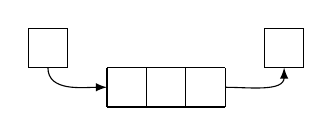
\begin{tikzpicture}[scale=0.5]
        \draw (0,0) grid (3,1);
        \draw (-2,1) grid (-1,2);
        \draw (4,1) grid (5,2);
        
        \draw[->,>=latex] (-1.5,1) to[out=270,in=180] (0,0.5);
        \draw[->,>=latex] (3,0.5) to[out=0,in=270] (4.5,1);
        \end{tikzpicture}
        \captionof{figure}{Enfiler - défiler}
   \end{center} 

\end{frame}
\begin{frame}
    \frametitle{}

    \begin{center}
    

        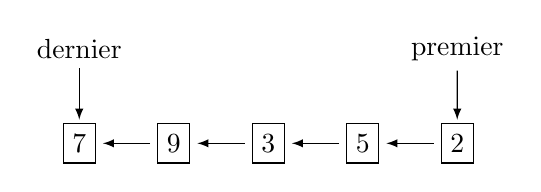
\begin{tikzpicture}[scale=0.6]
            \foreach \v/\x in {2/8,5/6,3/4,9/2}{
            \node[draw,minimum height=0.5cm] at (\x,0) {\v};
            \draw[->,>=latex] (\x-.5,0) -- (\x-1.5,0);
            }  
            \node[draw,minimum height=0.5cm] at (0,0) {7};
            \node (p) at (8,2) {premier};
            \draw[->,>=latex] (p) -- (8,0.5);
            \node (d) at (0,2) {dernier};
            \draw[->,>=latex] (d) -- (0,0.5);
        \end{tikzpicture}
        \captionof{figure}{Implémentation}
    \end{center}
\end{frame}
\begin{frame}
    \frametitle{Interface d'une file}

    \begin{itemize}
        \item \texttt{\textbf{creer\_file() $\rightarrow$ File()}}: crée une file vide.
        \item \texttt{\textbf{est\_vide(f: File) $\rightarrow$ bool}}: renvoie \textbf{\texttt{True}} si la file est vide, \textbf{\texttt{False}} sinon.
        \item \texttt{\textbf{enfiler(f: File, e: T) $\rightarrow$ None}}: ajoute un élément \emph{e} à l'arrière de la file.
        \item \texttt{\textbf{defiler(f: File) $\rightarrow$ T}}: retire et renvoie l'élément de l'avant de la file.
        \end{itemize}

\end{frame}
\begin{frame}
    \frametitle{Implémentation}

    \begin{itemize}
        \item \texttt{\textbf{creer\_file() $\rightarrow$ File()}}
        \item \texttt{\textbf{est\_vide(f: File) $\rightarrow$ bool}}
        \item \texttt{\textbf{enfiler(f: File, e: T) $\rightarrow$ None}}
        \item \texttt{\textbf{defiler(f: File) $\rightarrow$ T}}
        \end{itemize}

        \begin{activite}
            \begin{enumerate}
                \item \underline{Adapter l'interface} présentée pour créer une classe \textbf{\texttt{File}}. Il est nécessaire de maintenir deux attributs: \textbf{\texttt{premier}} et \textbf{\texttt{dernier}}. Il faudra également réutiliser la classe \textbf{\texttt{Element}}.
                \item \textbf{Pour les plus avancés:} Implémenter la méthode \textbf{\texttt{\_\_str\_\_}} qui affiche le contenu de la file.
            \end{enumerate}
        \end{activite}
\end{frame}
\begin{frame}[fragile]
    \frametitle{Correction}

\begin{lstlisting}[language=Python , basicstyle=\ttfamily\small, xleftmargin=2em, xrightmargin=2em]
class File:
    def __init__(self):
        self.premier = None
        self.dernier = None

    def est_vide(self) -> bool:
        return self.premier is None
\end{lstlisting}

\end{frame}
\begin{frame}[fragile]
    \frametitle{Correction}

\begin{lstlisting}[language=Python , basicstyle=\ttfamily\small, xleftmargin=2em, xrightmargin=2em]
def enfiler(self, e: int) -> None:
    nouveau = Element(e, None)

    if self.est_vide():
        # 1 seul élément: le premier est le dernier
        self.premier = nouveau
    else:
        # le dernier devient avant-dernier
        self.dernier.successeur = nouveau

    # le nouveau devient dernier
    self.dernier = nouveau
\end{lstlisting}

\end{frame}
\begin{frame}[fragile]
    \frametitle{Correction}

\begin{lstlisting}[language=Python , basicstyle=\ttfamily\small, xleftmargin=1em, xrightmargin=1em]
def defiler(self) -> int:
    if not self.est_vide():
        res = self.premier.donnees
        self.premier = self.premier.successeur
        return res
\end{lstlisting}

\end{frame}
\begin{frame}[fragile]
    \frametitle{Correction}

\begin{lstlisting}[language=Python , basicstyle=\ttfamily\small, xleftmargin=2em, xrightmargin=2em]
def __str__(self):
    c = self.premier
    s = ""
    while not c is None:
        s = s + str(c.donnees)+"|"
        c = c.successeur
    return "\u2BA4|" + s[:] + "\u2BA0"
\end{lstlisting}

\end{frame}
\begin{frame}[fragile]
    \frametitle{}
    \begin{center}
\begin{lstlisting}[language=Python , basicstyle=\ttfamily\small, xleftmargin=2em, xrightmargin=2em]
from random import randint

a = File()
for i in range(6):
    a.enfiler(randint(1, 20))
    print(a)

for i in range(6):
    a.defiler()
    print(a)
\end{lstlisting} 
    \captionof{code}{Affichage de la file}
    \label{CODE}
    \end{center}  

\end{frame}
\section{Ordonnancement}
\begin{frame}
    \frametitle{Ordonnancement}
\begin{aretenir}[]
Plusieurs algorithmes d'ordonnancement utilisent une file.
\end{aretenir}
\begin{center}
    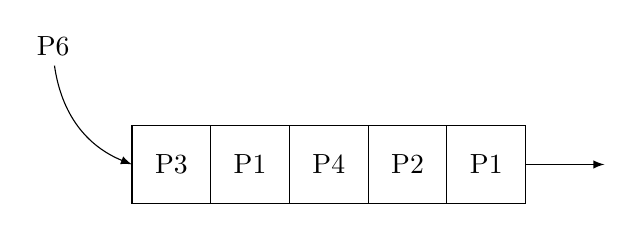
\begin{tikzpicture}
    \draw (0,0) grid (5,1);
    \foreach \x/\y in {0/P3,1/P1,2/P4,3/P2,4/P1}
    {
        \node at(.5+\x,.5) {\y};
    }
\node (p6) at(-1,2){P6};
    \draw[->,>=latex] (5,.5) -- (6,.5);
    \draw[->,>=latex] (p6) edge[bend right] (0,.5);

    \end{tikzpicture}
    \captionof{figure}{First Come First Served}
\end{center}

\end{frame}
\begin{frame}

\begin{center}
    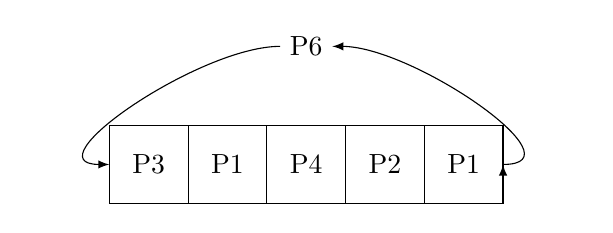
\begin{tikzpicture}
    \draw (0,0) grid (5,1);
    \foreach \x/\y in {0/P3,1/P1,2/P4,3/P2,4/P1}
    {
        \node at(.5+\x,.5) {\y};
    }
\node (p6) at(2.5,2){P6};
\draw[->,>=latex] (5,.5) edge[out=0,in=0] (p6);
\draw[->,>=latex] (p6) edge[out=180,in=180] (0,.5);

    \end{tikzpicture}
    \captionof{figure}{Round Robin}
\end{center}
Une \emph{quantum} de temps est alloué à chaque processus. Un processus qui n'est pas terminé retourne en fin de file.
\end{frame}
\end{document}